%%%%%%%%%%%%%%%%%%%%%%%%%%%%%%%%%%%%%%%%%%%%%%%%%%%%%%%%%%%%%%%%%%%%%%%%%%%%%%%%
%2345678901234567890123456789012345678901234567890123456789012345678901234567890
%        1         2         3         4         5         6         7         8

\documentclass[letterpaper, 10 pt, conference]{ieeeconf}  % Comment this line out
                                                          % if you need a4paper
%\documentclass[a4paper, 10pt, conference]{ieeeconf}      % Use this line for a4
                                                          % paper

\IEEEoverridecommandlockouts                              % This command is only
                                                          % needed if you want to
                                                          % use the \thanks command
\overrideIEEEmargins
% See the \addtolength command later in the file to balance the column lengths
% on the last page of the document

\usepackage{graphicx}
\usepackage{subfigure}
\usepackage[]{units}
\usepackage{url}

\title{\LARGE \bf
Analysis of Current Data Mining Techniques on SMS Spam Filtering
%I Got Them Research Paper Writing Blues...
%Intoxicated Cells: a Prospective Study of the Effects of Tequila on Pluripotent Stem Cells
}

\author{William Marshall$^1$%
%\thanks{*This work was supported by SUNFEST}% <-this % stops a space
\thanks{$^2$Lehigh University, USA {\tt\small wcm214@lehigh.edu}}
}

\begin{document}
\maketitle
\thispagestyle{empty}
\pagestyle{empty}


%%%%%%%%%%%%%%%%%%%%%%%%%%%%%%%%%%%%%%%%%%%%%%%%%%%%%%%%%%%%%%%%%%%%%%%%%%%%%%%%
\begin{abstract}
The necessity of a fast, accurate, easily trainable spam detection
system is reflected in the current proliferation of SMS spam
messages. By taking advantage of the suite of machine learning
algorithms integrated into WEKA, we provide an analysis of SMS spam
detection accuracy across severak different learning models, and
present the Naive Bayes algorithm as a primary choice.
\end{abstract}


%%%%%%%%%%%%%%%%%%%%%%%%%%%%%%%%%%%%%%%%%%%%%%%%%%%%%%%%%%%%%%%%%%%%%%%%%%%%%%%%
\section{INTRODUCTION}
Short Message Service (SMS) messages are one of the primary means of
communication. Between the years of 2007 and 2010, the number of sent
SMS messages tripled, and the global rate of message sending increased
to 200,000 texts per second [1]. Along with the increased usage of SMS
messages, the proportion of SMS spam messages has also not only risen
to match the new levels of traffic, but has accelerated to the point
where parts of Asia classified 30\% of all SMS messages as spam in
2012 [2]. Although SMS spam is not as prevelant as email spam -- which
constituted 70.7\% of all emails in Q2 2013 -- there is still a strong
motivation for cellular companies to employ effective spam detection
systems, since it's likely that customers are willing to pay more for
a service that is insulated from spam.

Many modern approaches to spam detection are founded upon the research
that stems from the identification of email spam. Email spam detection
benefits from features such as a subject header, initial greetings,
and the IP address of the sender. Such features are not applicable to
SMS messages which have an upper limit of 160 characters, providing
overall less information to perform classification. Additionally,
since SMS spam is less pervasive than email spam, its classification
is made more difficult due to the lower prior probability. Blanzieri
at al. were able to achieve an email spam misclassification rate of
only 1.17\% [3], which is a daunting task for SMS spam detection.

The differences between SMS and email spam detection warrant a
reevaluation of the effectiveness of current learning models. Fortunately, the University of Waikato has provided WEKA: a toolkit that conveniently provides implementations of many well known and vetted classification, association, and clustering techniques. The algorithms included in WEKA and tested in this paper are by no means an exhaustive analysis of the spam detetion literature, yet this paper should function well as an introduction for those who are new to machine learning, WEKA, and spam detection.

\section{Related Work}
Factory automation typically relies on careful environment control and
predictable inputs. Industrial perception has historically relied on
2D visual sensing where vision sensing is required
\cite{NIST2012:BinPicking}. This state of affairs is changing as
general purpose robots lead the shift to less structured environments,
a greater variety of behaviors, and full 3D perception and planning.

Recent approaches to perception for manipulation has moved beyond
standard 2D image processing by applying a variety of new sensing
modalities to the problem. A multi-flash camera sensor has been used
to observe depth edges of parts piled in a bin
\cite{Liu2012:BinPicking}. This work focused on fine manipulation in a
highly cluttered environment, and was able to achieve a 94\% success
rate with just under one second spent on object pose
estimation. Object recognition and pose estimation in complex, noisy
scenes is also demonstrated in \cite{Papazov2012:Grasping} by relying
on an RGB-D sensor.

An example of a responsive general purpose robotic platform
interacting with moving objects may be found in
\cite{Birbach2011:Catch}, in which a mobile humanoid robot is given
the ability to catch balls tossed toward it. This application requires
great care and attention be given to processing time, as being late is
not an option. In this case, the software performs real-time circle
detection at \unit[35]{ms} per image.

The aforementioned PR2 has been used extensively in tabletop
manipulation research \cite{WGObjectManipulation}. This work focused
on reliability and modularity, and has been demonstrated to enable the
PR2 to pick up a variety of objects, including those previously
unknown to the software.

Raw performance of perception for manipulator planning was a primary
consideration in \cite{Wagner2013:GPUMotionPlanning}, in which a
signed truncated distance field computed from Kinect data on a
high-end GPU is used to drive manipulator planning. The result is the
ability of a manipulation system to execute a planned, collision free
path three seconds after first exposure to the scene.

\section{Perception}
\begin{figure}[t]
\centering
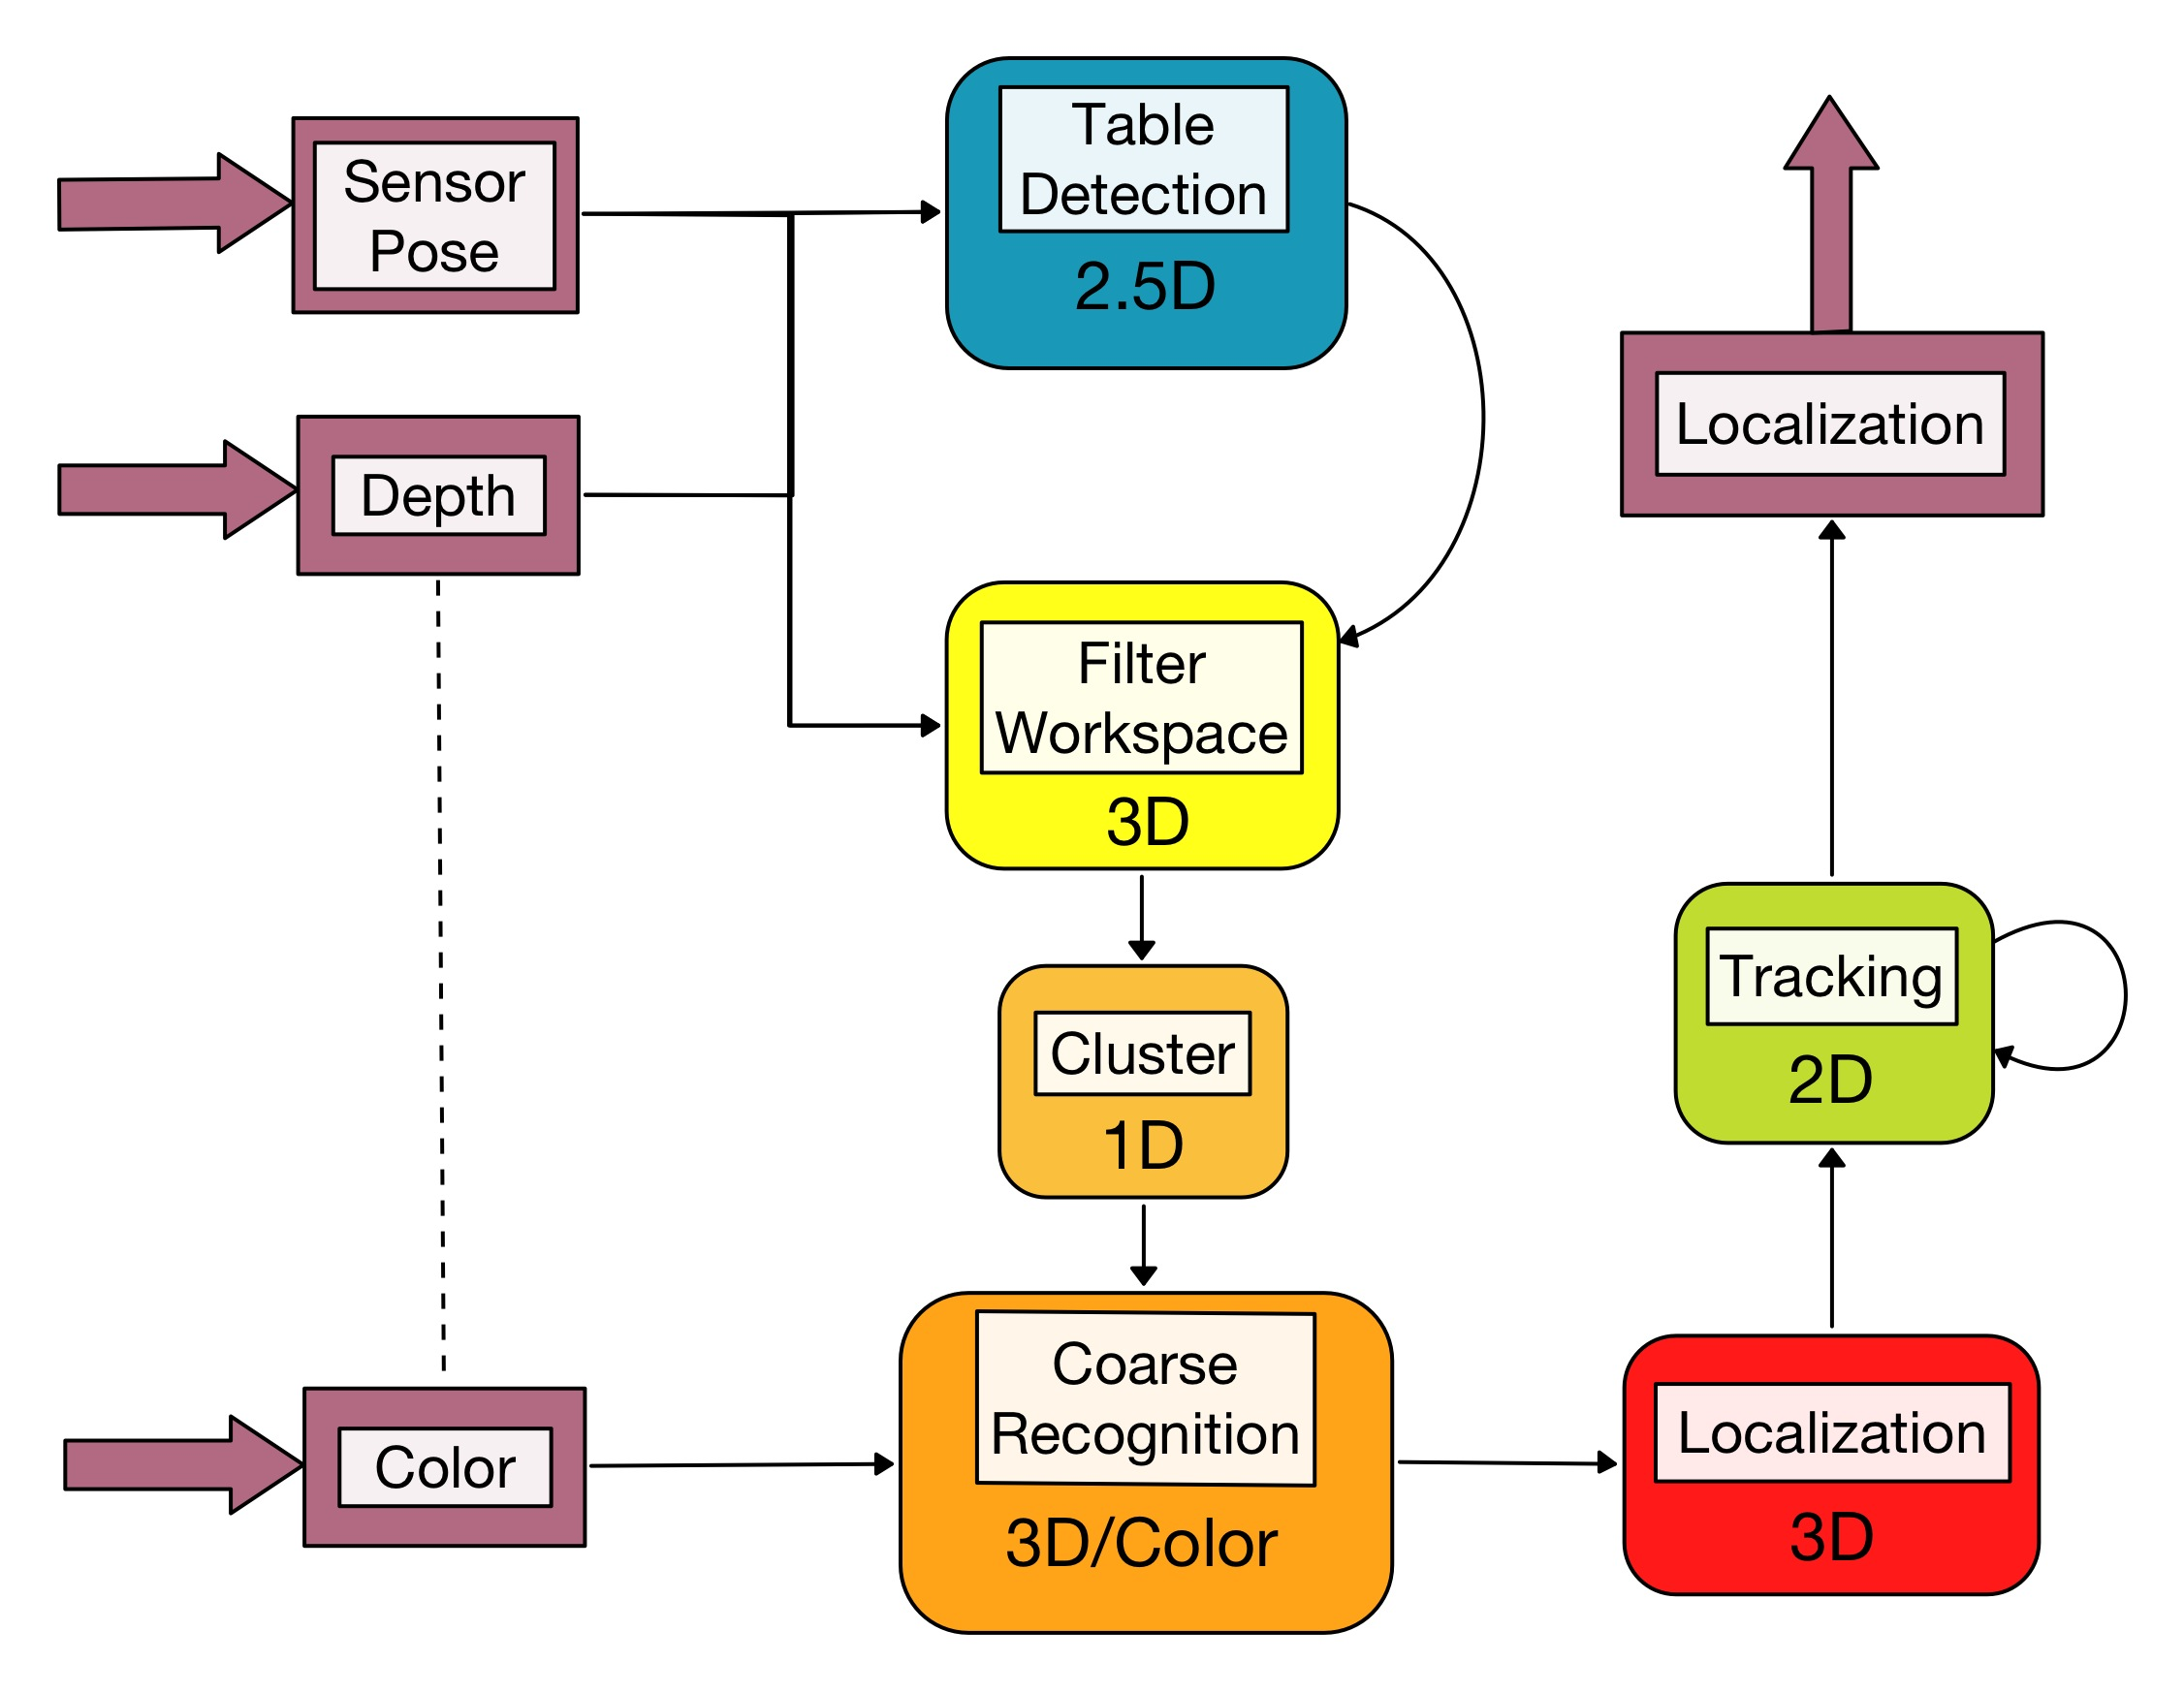
\includegraphics[width=0.9\columnwidth]{figures/perception-pipeline.jpg}
\caption{ The perception system is driven by registered depth and
  color images paired with an estimate of the RGB-D sensor's pose in
  the robot's coordinate frame. The dimensionality of the data
  processed by each stage is indicated in the figure, illustrating
  places where dimensionality reduction is used to improve efficiency.
}
\label{fig:perception-pipeline}
\end{figure}

The perception system employed here is made up of a staged processing
pipeline based on RGB-D sensor data, and the PR2's own pose
estimation, Figure~\ref{fig:perception-pipeline}. The system is given
information about objects of interest at startup, then takes its input
from ROS, and publishes localized, identified objects as they are
detected. The overall procedure is that table geometry is extracted to
perform an initial interpretation of the scene that disregards a large
fraction of sensor data. Detected points that lie above the work
surface are clustered, and those clusters are recognized and localized
to provide a pose estimation of identifiable objects. The individual
components of the perception pipeline are described in detail below.

\subsection{Conventions}
The robot coordinate frame is used to identify features of the system
and the environment in the following discussion. The convention
followed is that common to ROS: a right-handed coordinate system with
the X axis extending forward from the robot, the Y axis extending to
the robot's left, and the Z axis extending up from the base. Objects
may be positioned anywhere on the table surface, and are free to
rotate about their vertical axes.

\subsection{Work Surface Extraction}
\label{sec:table-detection}
During execution, the table height, direction, and extents are
periodically re-estimated from direct observation. This process is run
every ten seconds to allow for robot movement during operation without
requiring a reset of the system. In this stage, we search for a
connected component of the depth image that is dominated by points
within a narrow range of heights above ground level using a recursive
histogram analysis.

The inliers of a successful analysis -- consisting of a significant
fraction of points within \unit[2]{cm} of each other when projected
onto the Z axis -- are then used to extract the table orientation and
extents which are used in subsequent object extraction. Assuming
asymmetric geometry, the table orientation is calculated as the
eigenvector corresponding to the largest magnitude eigenvalue of the
covariance matrix of the inlier points projected onto the XY
plane. When a new table estimate is computed, it is atomically swapped
into a memory cell referenced at the start of each new object
detection update.

\subsection{Coarse Recognition and Localization}
Upon arrival of a pair of registered depth and color images, all
points not within a space above the table geometry previously
extracted are immediately removed. The remaining points are projected
onto the line corresponding to the table direction, and clustered
using a histogram analysis. These clusters are then run through
multiple coarse classifiers that use color statistics and size limits
to reject obvious object type mismatches. For instance, if a cluster
has a vertical extent of only \unit[10]{cm}, it will not be identified
as an object expected to be \unit[30]{cm} tall.

Multiple coarse recognizers corresponding to the known object
vocabulary may support any given cluster. All clusters recognized by
at least one coarse recognizer have their centroids computed, and are
fed forward in the system. When no coarse recognizer fires, this
processing stage provides an opportunity for early exit.

\subsection{Refined Recognition and Localization}
The objects to be recognized and localized must be modeled before the
system will identify them as anything other than unknown obstacles. A
point cloud of an object's surface is first captured, then used to
construct a truncated distance field representing a uniform sampling
of a cost function whose minimal manifold corresponds to the surface
of the object model. This sampling is computed by performing a
Euclidean distance transform (EDT) on a voxel grid populated from the
model point cloud. This preprocessing step is efficiently performed
across multiple CPU cores using the approach described in
\cite{Meijster2002}.

Observed point clusters are recognized by finding a 2D transformation
that minimizes this cost function when summed over all observed
points. This approach is similar to \cite{Papazov2011:Stochastic}, but
the nonlinear optimization technique employed here is Powell's dogleg
method \cite{Powell1964}. The optimization procedure iteratively
evaluates 2D transformations applied to 3D points whose transformed
coordinates are used to index into the sampled cost function until a
local minimum is found.

% The optimization procedure is an iterative
% evaluation of parameters that converges to a local minimum. In
% concrete terms, what is involved is the transformation of 3D points on
% a 2D surface, which are then used to index into the sampled cost
% function given by the distance field associated with an object model.

The necessary arithmetic and memory access patterns for this operation
lie squarely within the core competencies of hardware designed for
graphics acceleration. By loading the sampled cost function into a 3D
texture in OpenGL, the cost of each transformed point is obtained by
looking up a floating point value in a texture. The graphics
processing unit (GPU) is used to perform linear interpolation along
each axis of this texture lookup to further smooth the search space,
and texture coordinates are clamped to truncate the cost function out
to infinity, thereby mitigating the deleterious effects of outliers.

First, the image coordinates of the relevant points are translated to
a cropped coordinate frame containing only the observed points. These
coordinates are then paired with the 3D points reconstructed from the
depth data, transformed into the object's coordinate frame using the
points' centroid as the origin, and loaded onto the GPU. The 2D
projection of the original data is used to address the output data as
it is, by construction, an injective mapping from 3D points to 2D
coordinates.

A GLSL vertex shader applies the candidate transformation, while
passing through the 2D coordinates for each point unchanged. The
fragment shader looks up the distance value from the cost function
texture, and writes the interpolated value it arrives at to that
point's location in the cropped 2D coordinate frame. Additionally, the
optimization procedure lends itself to a batch interface, wherein
several choices of parameters are evaluated in an overlapping fashion,
thereby allowing the GPU to compute cost function evaluations while
asynchronously transferring the results of previous evaluations back
to the CPU.

When the optimization process has finished, the average distance from
each point in the observation under the minimal-cost transformation to
the object model is considered to determine if we have a successful
identification. Multiple optimizations may be performed to resolve the
ambiguity of multiple coarse recognizers positively identifying point
cluster summaries. An additional gain in efficiency is found by
considering the rotational symmetry of each object. The general
problem of identifying a 2D translation and 1D rotation is, for
example, reduced to just the 2D translation optimization for objects
that are fully symmetric. The rotational symmetry of each object is
therefore recorded along with the object model information used by the
coarse recognition step.

\subsection{Tracking}
The above process is applied to a small number of observed point
clusters, while the rest are left as unidentified. All clusters are
then passed to a tracking component that models the kinematics of both
identified and unidentified point clouds. Observation integration is
achieved by maintaining a track state that includes both object
position and velocity in a Kalman filtering framework.

Inspired by the linear arrangement of objects on a long table when
viewed from off-axis, observations are aligned with existing estimates
using the Needleman-Wunsch optimal matching algorithm
\cite{NeedlemanWunsch1970}. This algorithm provides a principled way
to match predictions of a linear chain of states to observations while
taking potential object identification as well as position into
account. This mechanism supports the presence of multiple objects
within a single view by matching observations to existing tracks, or
determining that an observation necessitates the initialization of a
new track.

% In the usual application of this algorithm to string
% alignment, \textit{skip} characters may be added at any point in one
% or the other strings. These are points at which two strings do not
% align, but whose removal from one string allows a likely match to
% continue beyond the missed location. The algorithm thus prevents us
% from aligning a track identified as one object with an observation
% identified as a different object type, and provides the necessary
% mechanism to inject new tracks and deal with data dropout.

The motion model used for tracking is one of zero
acceleration. Furthermore, we are interested in the problem of
tracking objects undergoing identical motion. We take advantage of
this commonality by initializing the position covariance estimate of a
new track by a sensor noise model as is usual, but carry over both
velocity value and covariance from previous tracks. This causes the
velocity estimate of successive tracks to adhere very tightly to a
robust running average.

Final reporting from the tracker is governed by a configuration
parameter indicating how many observations of any given track are
needed before reporting is warranted. When a recognized object track
is reported, an estimate of its position on the table plane is
extracted from the Kalman filter, and a bounded history of orientation
estimates provided by the localization optimization is passed through
a RANSAC \cite{Fischler1981:RANSAC} procedure to compute a robust
mean. The special consideration given to object yaw is due to the
expectation that yaw measurements will be the noisiest axis of
observation due to varying geometry occlusion as the view of an object
changes over time. Consider, for example, a round watering can with a
long spout. The yaw estimate for such an object will likely be much
better when computed from views in which the spout is visible than
those where it can not be seen.

% If the spout is not visible from some views, the yaw estimate
% is likely to be much less accurate than that estimated from views that
% capture at least part of the spout geometry.

% \item Object clustering: When looking down on objects with overhanging
%   geometry, we found that connected depth components weren't the best
%   model for the point clouds associated with each object. Histogram
%   objects along the table's long axis.

\section{Manipulation}

When an object is detected, the pick-and-place manipulation pipeline
gets called to pick up the approaching object and move it to a desired
location. The manipulation pipeline is comprised of three main
components, namely grasping, motion planning and execution. Before the
pipeline is called, an arm is chosen to pick up the object. Currently
we are simply alternating between the arms. If no feasible grasps for
the first arm are computed, we have found that quite often the other
arm is capable of performing the pick-and-place action after receiving
the next observation.

Note, that the same system is used for manipulating both static and
dynamic objects. In the case of the static object, the entire pipeline
just executes immediately, instead of waiting for the object to enter
the robot's workspace.

\subsection{Grasping}

Reliable grasping of a static object by a robot's end-effector can be
a difficult task given the uncertainty in each part of the system,
from the object pose estimation to the robot's mechanical
calibration. Additional problems arise when the object is moving at a
fast speed. To simplify grasp planning, we exploit the fact that we
have a well-defined set of objects to be manipulated. This allows us
to restrict the set of grasps for each type of object to ones that we
have previously tested and saved in a database. Once an object is
detected, the grasps are retrieved and checked for feasibility. We
will now explain each component of the grasp selection process.

\textit{\textbf{Types of Grasps.}}
The process of picking up an object requires the end-effector to move between three different 6-DOF poses:
\begin{itemize}
\item \textit{pregrasp -} An end-effector pose that is offset from the object (see Figure~\ref{fig:recording_grasps-photo}, left). The motion planner is used to plan a collision free trajectory from the arm's waiting configuration to a valid configuration with the end-effector at the pregrasp pose.
\item \textit{grasp -} The pose of the end-effector in which its fingers are in position to reliably enclose part of the object (see Figure~\ref{fig:recording_grasps-photo}, middle).
\item \textit{postgrasp -} The end-effector pose after it moved away from the surface with the object grasped. The motion planner is then used to compute a feasible motion for the arm that takes the end-effector from the postgrasp to the desired place location.
\end{itemize}

\textit{\textbf{Recording Grasps.}}  Prior to manipulating a new
object, we create a set of grasps for it. We found the grasp recording
process to be simple and reliable. The process begins by placing the
object within the workspace of either one of the arms and within the
RGB-D sensor's view. Once the item is localized, the user is asked to
move the end-effector to the desired pregrasp pose and the 6-DOF pose
of the end-effector in the coordinate frame of the object is
recorded. The process is repeated for the grasp pose, and the two
grasps are then added to the grasp database for that object type. This
pair of grasps defines a collision trajectory that brings the end
effector into contact with the target object. The angle of this
trajectory is chosen to improve the chances of a mechanically stable
grip. In general, we found that a single set of postgrasp positions
can be used for all object types so the user is not required to record
a postgrasp for each object.  Instead, the grasp orientation is paired
with a set of postgrasp translations above the object for each object
type. In our experiments, the set of grasps for each object contains
between two and twenty pregrasp-grasp pairs. See
Figure~\ref{fig:recording_grasps-photo} for an example.

\begin{figure}[t]
\centering
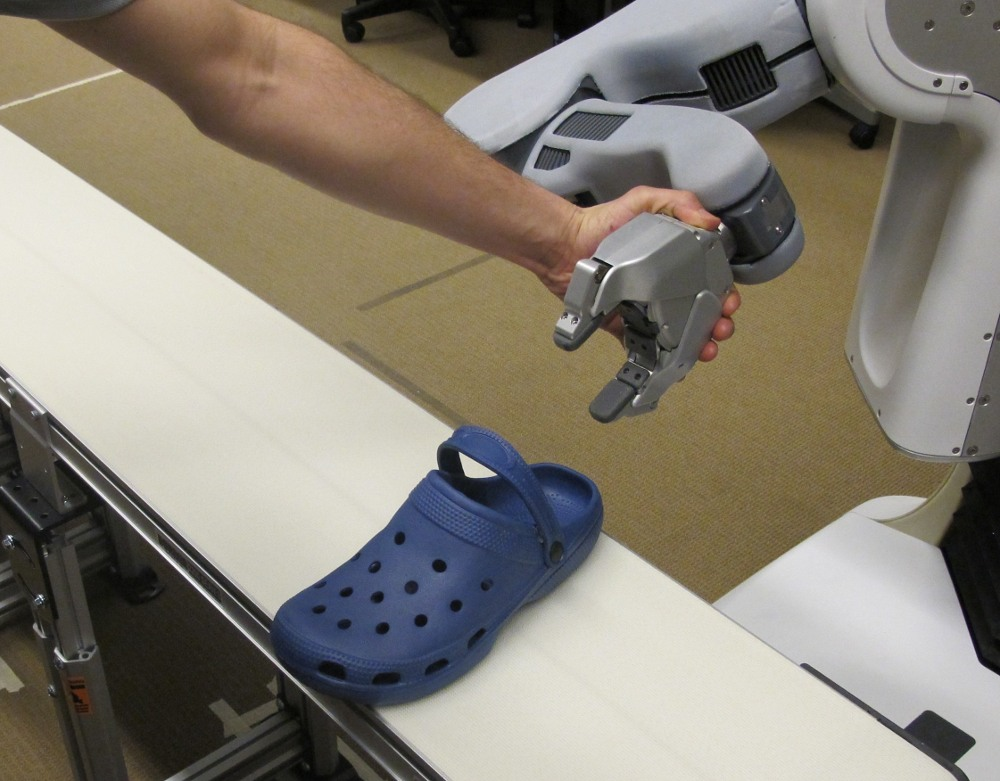
\includegraphics[width=0.31\columnwidth]{figures/croc-record_pregrasp.jpg}
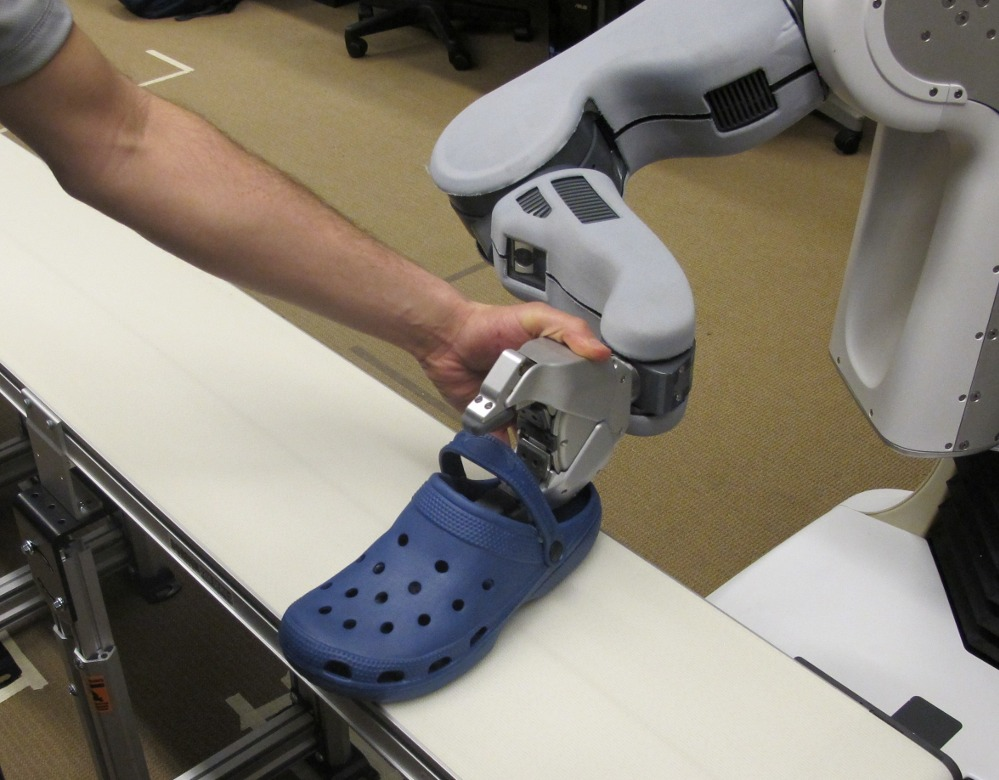
\includegraphics[width=0.31\columnwidth]{figures/croc-record_grasp.jpg}
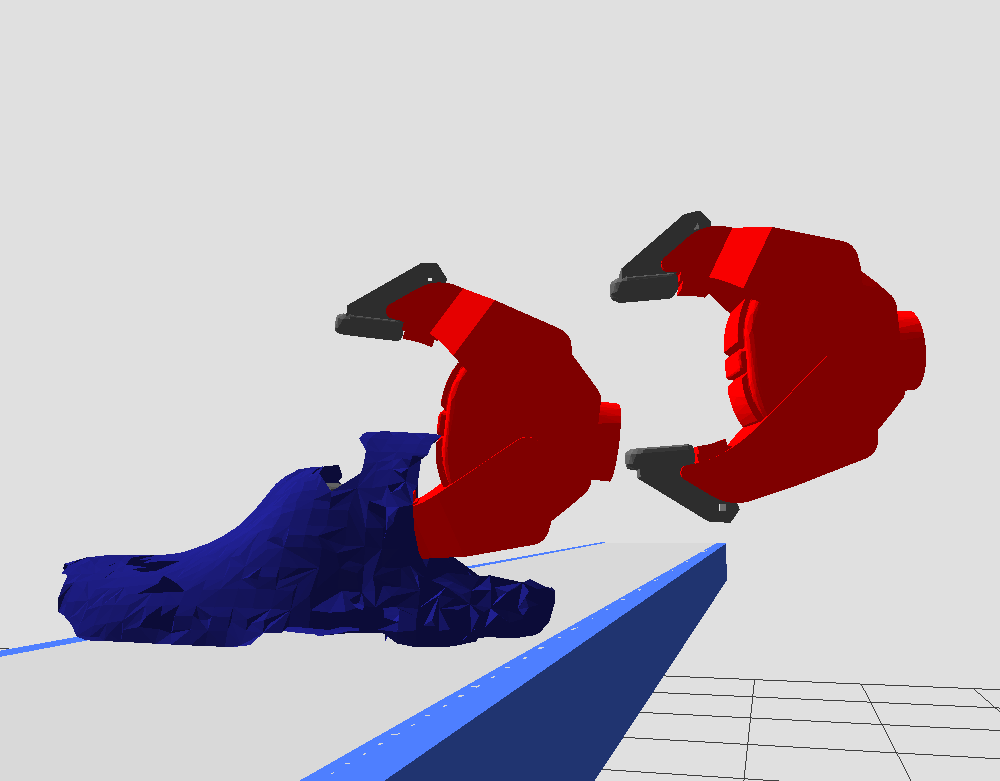
\includegraphics[width=0.31\columnwidth]{figures/croc-grasps-outside_view.png}
\caption{
From left to right, the user moves the end-effector to the pregrasp pose and then to the grasp pose. The pair of grasps is added to the database as they appear on the right.
}
\label{fig:recording_grasps-photo}
\end{figure}

\textit{\textbf{Grasp Selection.}}  Upon detection of a new object, we
use its estimated pose and velocity to predict $t_{pred}$ and
$x_{pred}$. $t_{pred}$ is the time at which the object will be at the
center of the workspace of the arm and $x_{pred}$ is the predicted
6-DOF object pose in the world. The object type is used to retrieve a
set of pregrasps and grasps from the database. For each pregrasp,
$p_i$, we use $x_{pred}$ to compute $x_{p_i}$, the pregrasp pose in
the world frame for when the object will be at its predicted pose. The
same is done for each grasp $g_i$ to compute $x_{g_i}$.

Before we add $\{x_{p_i}, x_{g_i}\}$ to $X_{pg}$, the set of feasible
pregrasp-grasp tuples, the following two feasibility checks are
performed on each tuple:
\begin{itemize}
% \item \textit{chase grasps -} It is very difficult to pick up a moving
%   object using a grasp motion that is \textit{chasing} it along the
%   direction of its velocity, $v_{object}$.  It rarely succeeds if
%   $v_{object}$ is equal to or greater than the maximum speed of the
%   end-effector along the grasp motion. Thus, we chose to filter out
%   the chase grasps completely by detecting if the pregrasp to grasp
%   motion is moving in the same direction as $v_{object}$. We do this
%   by computing $c = \|v_{object}\| \cdot \|x_{g_i}\|$. If $c <
%   k^\circ$, the tuple is deemed too similar to the object's velocity
%   and it is rejected. In our experiments, we set $k$ to correspond to
%   an angular difference of $-30^\circ$.
\item \textit{chase grasps -} It is very difficult to pick up a moving
  object using a grasp motion that is \textit{chasing} it along the
  direction of its velocity, $v_{object}$.  It rarely succeeds if
  $v_{object}$ is equal to or greater than the maximum speed of the
  end-effector along the grasp motion. Thus, we chose to filter out
  the chase grasps completely by detecting if the pregrasp to grasp
  motion is moving in the same direction as $v_{object}$. We do this
  by computing $c = \frac{v_{object} \cdot (x_{p_i} -
    x_{g_i})}{\|v_{object}\|\|x_{p_i} - x_{g_i}\|}$. If $c <
  k^\circ$, the tuple is deemed too similar to the object's velocity
  and it is rejected. In our experiments, we set $k$ to correspond to
  an angular difference of $-30^\circ$.

 
\item \textit{kinematics -} We check if each $x_{p_i}$ and $x_{g_i}$
  is kinematically feasible for the arm of the robot using an inverse
  kinematics solver to compute the corresponding joint
  configuration. If either is invalid, the tuple is rejected. In
  Figure~\ref{fig:kinematics_feasibility_check}, six pregrasp-grasp
  tuples are shown for the basket. After they are checked for
  kinematic feasibility, the ones in red (darker color) are discarded
  because they are unreachable by the right arm.
\end{itemize}

\begin{figure}[t]
\centering
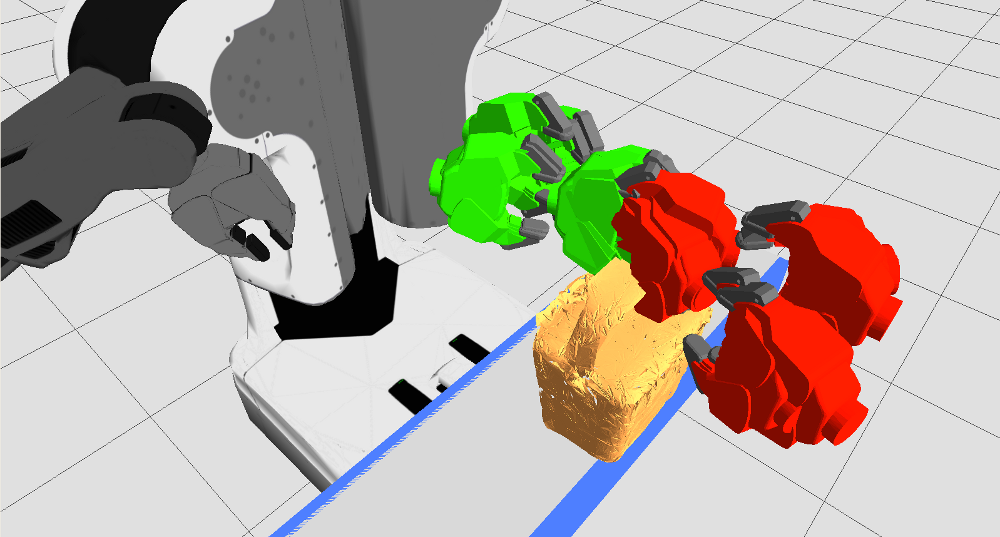
\includegraphics[width=\columnwidth]{figures/covered_basket-grasps-kinematics_check.png}
\caption{
The end-effectors in green are included in $X_{pg}$, while the ones shown in red are discarded by the kinematic feasibility check.
}
\label{fig:kinematics_feasibility_check}
\end{figure}

Given a set of valid grasps, a heuristic is typically used to select
the best grasp to plan for~\cite{WGGrasping}. However, this approach
can be overly restrictive, as the feasibility of the grasp depends on
the estimated time of arrival of the object. The better option is to
let the planner itself figure out which grasp to plan to given the
time constraint.
%a common approach to choosing which one to plan to, is to rank them using heuristics such as the number of sensed object points that fit inside the gripper or the distance from the object center~\cite{WGGrasping}. These heuristics are used because the grasp is planned on the fly and its quality is unknown. Given that our grasps were recorded previously, we are confident in their reliability and how to choose between them is unclear. 

% Thus, instead of choosing a single pregrasp-grasp tuple to target, the
% entire set of pregrasps in $X_{pg}$ is sent to the motion planner,
% allowing the planner to determine the $\{x_{p_j}, x_{g_j}\}$ in
% $X_{pg}$ that is feasible and optimizes costs well. After a plan is
% computed by the planner, the final waypoint of the planned path to the
% pregrasp, $x_{p_j}$, chosen by the planner. We use the corresponding
% grasp, $x_{g_j}$ as the grasp pose.

Thus, instead of choosing a single pregrasp-grasp tuple to target, the
entire set of pregrasps in $X_{pg}$ is sent to the motion
planner. When the planner finds a collision-free trajectory to an
element of $X_{pg}$, we select the corresponding grasp, $x_{g_j}$ as
the grasp pose. Computing the postgrasp is a straightforward process,
generic across object types. Given the grasp, $x_{g_j}$, we compute
the postgrasp, $x_{po_j}$, by searching through the set of postgrasps
for a kinematically feasible arm configuration that is as far from the
table as possible. In our experiments, we found that the $x_{po_j}$
chosen was typically within 12cm of $x_{g_j}$.

\subsection{Motion Planning}

% In an environment where robots work alongside people, it is important
% that the robot's behavior is consistent and predictable. This way, any
% human workers nearby can feel comfortable and safe around it. In
% particular, for a robot to be an effective member of a team on an
% assembly line that sorts moving objects into bins, the robot motions
% needs to be consistent, predictable and as close to optimal as
% possible in order for people to be able to work alongside and within
% the workspace of the robot. With this in mind, we implemented a
% heuristic search-based approach to generate motion plans for each of
% the robot's arms independently.

Heuristic searches such as A* provide strong theoretical guarantees
such as completeness and optimality or bounds on
suboptimality~\cite{Pearl-heur}. Their generality allows for complex
constraints and cost functions, while providing good cost minimization
and consistency in the solution. Consistency here implies that given
similar input, similar output is produced, thus making the robot's
motions more predictable.

Motion planning for pick-and-place of moving objects needs to be
performed as fast as possible so the robot has enough time to execute
the computed motions in time. To combat the high dimensionality of the
planning problem, we employ a heuristic search based approach that
uses an anytime variant of A* called ARA*~\cite{LikGorThr-ara} that
quickly finds an initial, and possibly sub-optimal, solution and
repairs it while deliberation time allows. The approach also relies on
a compact graph representation and informative heuristics to provide
real time performance. Details on this approach and applications to single and dual-arm motion planning can be found in~\cite{Cohen2, Cohen3}. 

We configured the planner to search in a 7 dimensional task space, $\{{x, y, z, roll, pitch, yaw, \theta}\}$, that represents the 6-DOF pose of the end-effector in the world frame, coupled with $\theta$, the position of the redundant degree of freedom in the robot's arm. This representation can be used when planning for a robot with one or more 7-DOF manipulators, such as the PR2 robot. In our experiments, we execute two independent instances of the planner, one for each arm. The cost function we use is aimed to minimize the 6-DOF path length of the end-effector.

During the pick action, the planner is called to plan a path from the \textit{waiting} configuration of the arm to one of the pregrasps in $X_{pg}$. Before planning begins, the geometry of the fixed objects in the robot's workspace are added to the collision representation. In our experiments, this included the conveyor belt and bins that surrounded the robot. After the robot grasps the object, the collision geometry of the object is attached to the robot's collision model. During the place action, a plan is requested from the postgrasp to any one of the drop poses above the bins. Note that there is nothing constraining the user from having the robot gently place the item on a surface instead. Now that a potentially fragile object (or an object filled with something) is grasped in the robot's end-effector, we impose an upright path constraint on the planner when computing a path for the place action. The constraint requires the planner to maintain the initial $\{roll, pitch, yaw\}$ of the end-effector throughout the path with a small tolerance in each dimension.
 
After a path is computed, we pass it through a simple deterministic shortcutting routine that can deal effectively with discretization artifacts. We found that only a single pass through the points was necessary. In our experiments, the entire shortcutting step lasted between 5-10ms, including checking the interpolated motions for collisions every $2^{\circ}$.

The ability to accurately predict the time it takes to execute a
trajectory is essential to picking up a quickly moving object. Being
that our motion planner plans solely for the kinematics of the arm, we
then perform a final post-processing step, in which the shortest
timing intervals between points are computed that enforce the robot's
dynamic constraints~\cite{IterativeSmoother}. The waypoint locations
themselves are not moved, instead feasible velocities and
accelerations are assigned. We found in our experiments that on
average, for a trajectory from an arm's initial configuration to a
pregrasp pose, the predicted execution timing and the actual
trajectory execution timing differ by approximately \unit[80]{ms}. The
pregrasp-to-grasp trajectory is much shorter, which provides for a
much smaller temporal prediction error, thus making the pregrasp pose
a useful waypoint at which to make final timing adjustments to achieve
a precise collision.

\subsection{Execution}

Given that the object is moving at a reasonable pace, the pick action
is substantially more difficult to execute than the place because very
precise timing is needed to succesfully pick up the object with a firm
grasp. For example, in our experiments the objects moved at
approximately \unitfrac[33]{cm\,}{\,s} across the robot's
workspace. At that velocity, if the execution of our grasp motion is
\unit[100]{ms} too late, the object will have passed $x_{pred}$ by
more than \unit[3]{cm}, and, depending on the type of the object, it
is very likely that the end-effector will swipe and miss.

\textit{\textbf{Pick Action.}} 
At this stage in the pipeline, it is confirmed that the entire pick action is kinematically feasible. In the case of the pick action, the following two trajectories have been generated:

\begin{itemize}
\item $traj_{p}$ - The pregrasp trajectory begins at the waiting configuration of the arm and ends at $x_{p_{j}}$. It is a collision free path generated by the motion planner, then shortcutted and filtered. $traj_{p}$ has a predicted trajectory execution duration of $d_{p_{pred}}$ seconds.
\item $traj_{g}$ - The grasp trajectory begins with the wrist at $x_{p_{j}}$, then moves to $x_{g_{j}}$ and ends at $x_{po_{j}}$. The path is an open loop motion in which the end-effector moves a very short total distance. $traj_{g}$ is filtered to assure the robot can execute it. Note that we define $d_{g_{pred}}$ as the predicted trajectory execution duration of the trajectory from the start until $x_{g_{j}}$. We disregard the execution time from $x_{g_{j}}$ to $x_{po_{j}}$ because the first half of the motion is the only time sensitive component, given that the end-effector has to be at $x_{g_i}$ to pick up the object at $x_{pred}$ at time $t_{pred}$.
\end{itemize}

The next step is to determine whether there is enough time for the
robot to execute both trajectories in time to pick up the object at
$t_{pred}$. The pickup is determined to be feasible if $t_{pred} >
(t_{now} + d_{p_{pred}} + d_{g_{pred}})$. If the pickup is feasible,
then $traj_{p}$ is executed immediatly. After it is completed,
$traj_{g}$ will begin execution at $t_{g_{execute}} = t_{pred} -
d_{g_{pred}}$. The end-effector is commanded to start closing as it is
approaching the grasp pose. In our experiments, we found that
depending on how early the object was detected and which arm is being
used, the robot would sleep for between 0.0 and 1.5 seconds between
executing the trajectories to ensure a well-timed grasp.


\textit{\textbf{Place Action.}}
After the object is grasped and raised to the postgrasp, there is not much work left to do. The computed path with the upright orientation constraint on the end-effector is executed immediatly. After the end-effector opens, allowing the object to drop into the desired bin, the arm returns to the waiting configuration. The purpose of the waiting configuration is two fold. First, it is intended to keep the arm that is closer to the feed edge of the belt out of the view of the RGB-D sensor, regardless of where the bins are located. Second, it is desirable to keep the arm in a configuration that is close to the table to aid in quicker reaction times by having to execute shorter trajectories.




\section{Experiments}

% We should have a \subsection{PR2 Robot} discussing the PR2. We should try to keep the paper as robot agnostic as possible and here we should have an introduction to our chosen mobile manipulation platform, the pr2.

\subsection{Computing Platforms}
All logic related to planning was executed onboard the PR2's own
computers. The perception software was hosted remotely on a desktop
computer with an Intel Core i7-2600 quad-core CPU at 3.4GHz and an
NVIDIA GeForce GT 420 GPU with 48 CUDA cores, a low-end graphics card
from 2010. The imposition of networking between these two critical
components adds a significant and variable amount of latency to the
system, however the PR2 used for these experiments did not have a
discrete GPU, and so could not host the perception system itself. The
perception pipeline was written in the Haskell functional programming
language, and compiled with the
GHC\footnote{\url{http://www.haskell.org/ghc}} 7.6.1 compiler.

\subsection{Object Selection}
\begin{figure}[t]
\centering
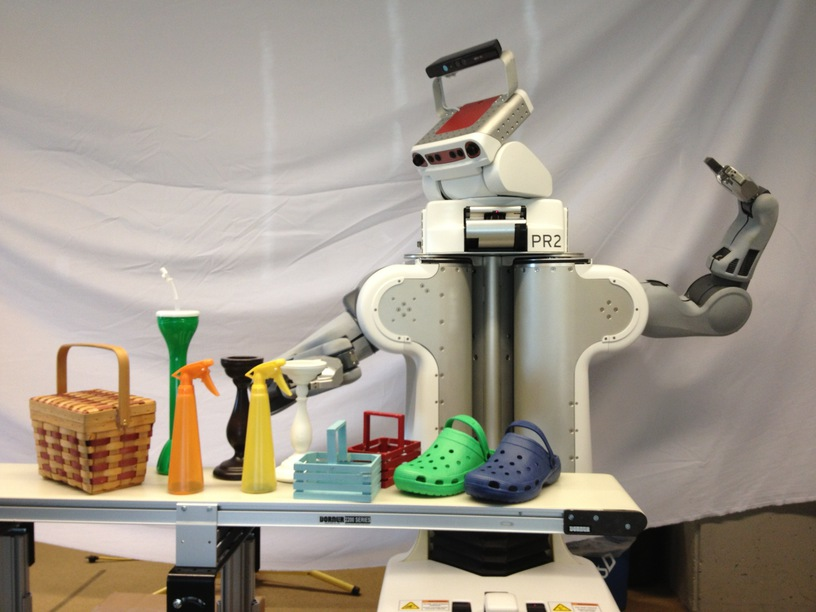
\includegraphics[width=0.8\columnwidth]{figures/object-group-photo-sm.jpg}
\caption{
The objects used for all experiments.
}
\label{fig:group-photo}
\end{figure}

The objects chosen, Figure~\ref{fig:group-photo}, range in height from
\unit[15]{cm} to \unit[45]{cm}, and breadth from \unit[8]{cm} to
\unit[25]{cm}. These objects also display a variety of rotational
symmetries, which affects their localization and how the objects may
be grasped. The candlesticks and tall green bottle have an infinite
order of rotational symmetry, denoted $C_\infty$, which translates to
a freedom to grasp such an object from any angle, and frees the
localization optimization from needing to consider object
orientation. The shoe is not rotationally symmetric, denoted $C_1$,
and must be grasped from its open end. The spritzer bottle is also
$C_1$, but may be grasped from either side to hook the PR2's fingers
underneath the overhanging geometry of the trigger mechanism. The
various baskets are all $C_2$, as their handles may be grasped from
either side.

Object models were acquired using RoboEarth software
\cite{DiMarco2012:RoboEarthModel}, a poster with fiducial markers, and
a Kinect sensor. The models gathered for the experiments described
here consist of 500 thousand to 1 million points.

\subsection{Pick-and-Place}
Figure~\ref{fig:group-photo} shows the conveyor belt used for testing
both static grasps, in which objects are placed on the surface in
front of the PR2 with the belt motor turned off, and dynamic grasps,
in which the belt motor is on. In the static grasp configuration, the
robot's head is oriented so that it is looking down at the table, and
objects are rapidly placed in front of it. As soon as the robot begins
to clear the work surface with an object in hand, a new object is
placed on the surface. Objects are placed such that at least one arm
can plausibly perform a grasp, but precise position and orientation
are allowed to vary within that constraint.

The experiment conducted in the static grasp configuration involved
100 pick-and-place operations in which the robot removes an object
placed onto the work surface in front of it, and places the object
into one of two bins placed on either side of it. Of the 100 attempted
actions, 91 were successful. The most common failure mode involved the
object slipping out of the robot's gripper due to an insecure
grasp. These 100 actions were timed in blocks of 10, yielding an
average of \unit[6.7]{s} per pick-and-place action. During the time
these experiments were conducted, the perception system failed to
identify an object before a two second timeout period elapsed on two
occasions. The experiments in which perception failed are not included
in the reported time, as we did not have a consistent approach to
failure recovery.

The dynamic configuration shown in the video associated with this
paper has the robot looking down the length of the conveyor belt, as
in Figure~\ref{fig:group-photo}. Objects are placed on the far end of
the \unit[2.13]{m} belt, and carried past the robot. In this
configuration, the perception system only reports on objects it has
seen a minimum of three times. This limits system responsiveness, but
is important to eliminate spurious observations of the object being
hand-placed on the end of the belt, and to ensure stability in pose
estimation.

System performance was measured over 100 pick-and-place operation
attempts with the belt at its top speed, \unitfrac[33]{cm\,}{\,s}, 87
of which were successful. Six objects were effectively ignored due to
the planner being unable to compute a suitable trajectory for either
arm in the allotted time. Of these six, five were spritzer bottles,
suggesting that the grasps chosen for this object did not leave the
planner enough freedom to maneuver. The seven other failures were
fumbled grasps. As in the static test, sometimes an insecure grasp
would lead to an object being dropped. The dynamic test added the new
failure mode of objects bouncing off of the back of the open gripper
during a catch attempt. This contribution of momentum to the
experiment was an excellent test of the system's overall timing: the
gripper had to close around the object as it hooked available geometry
in order to absorb all of its momentum without excessively
destabilizing the object. The tight timing constraints, paired with
the design of the PR2's arms, meant that the robot's arm farther from
where the objects were coming from was easier to utilize. Of the 94
attempted grasps, 57 were made by the far arm.

\section{Analysis}
\subsection{Perception Performance}
Preprocessing includes collecting a point cloud for each object to be
identified. The raw point data is used to populate a \unit[0.5]{cm$^3$}
resolution voxel grid, then passed through a Euclidean Distance
Transform (EDT), taking an average of \unit[304]{ms} for each object.

% \begin{figure}[t]
% \centering
% 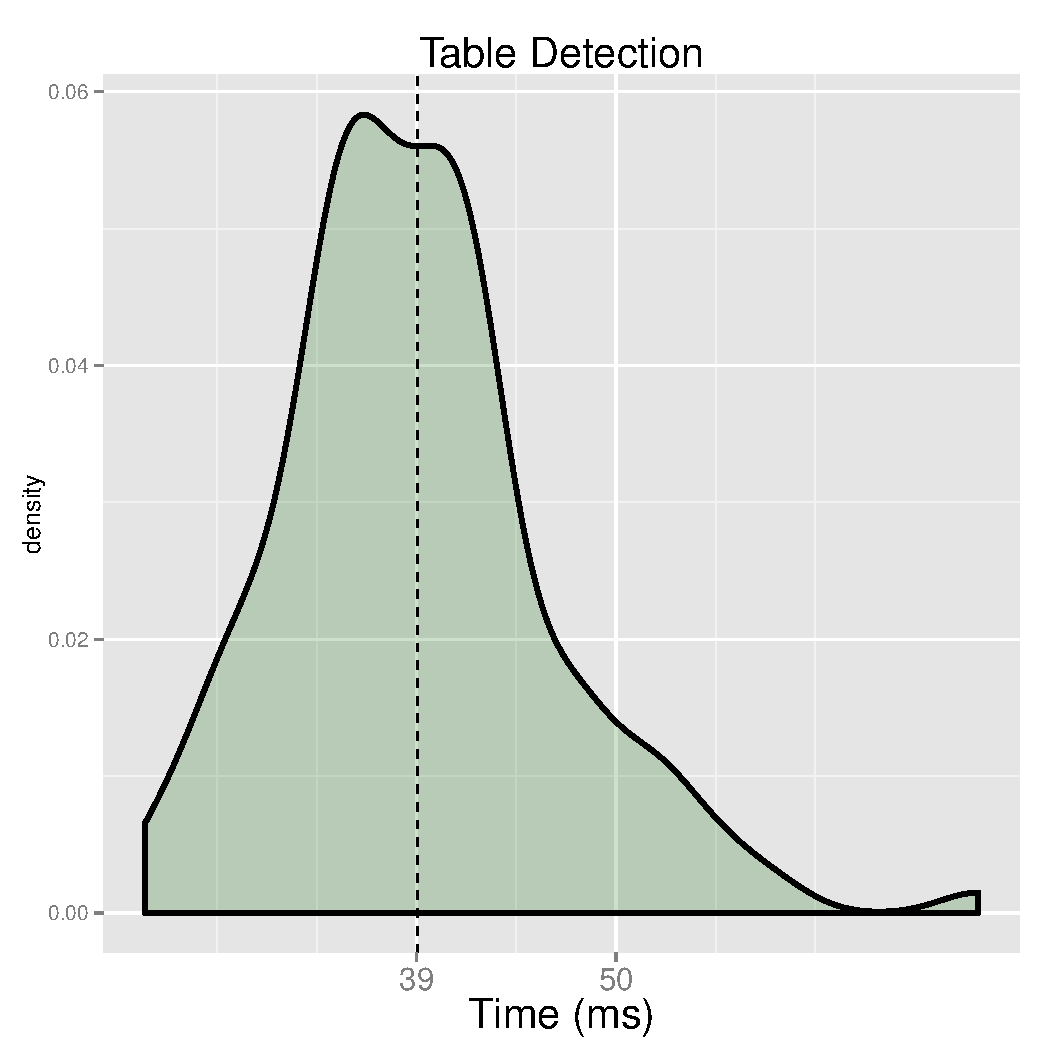
\includegraphics[width=0.8\columnwidth]{figures/table-density.pdf}
% \caption{
% Table extraction is performed with a recursive histogram over
% candidate connected components of the depth image.
% }
% \label{fig:table-density}
% \end{figure}

Once the system is running, parameters describing the conveyor belt
surface are periodically recalculated as described in
Section~\ref{sec:table-detection}. This process took an average of
\unit[39]{ms} per update, and was run concurrently with the rest of
the perception pipeline in a separate thread.

% Figure~\ref{fig:table-density}
% shows a kernel density estimate of overall table detection
% performance, with a mean processing time of 39ms. This process is run
% concurrently to the rest of the perception pipeline in a separate
% thread, and does not noticeably impact performance of the higher
% frequency components of the perception system.

\begin{figure}[t]
\centering
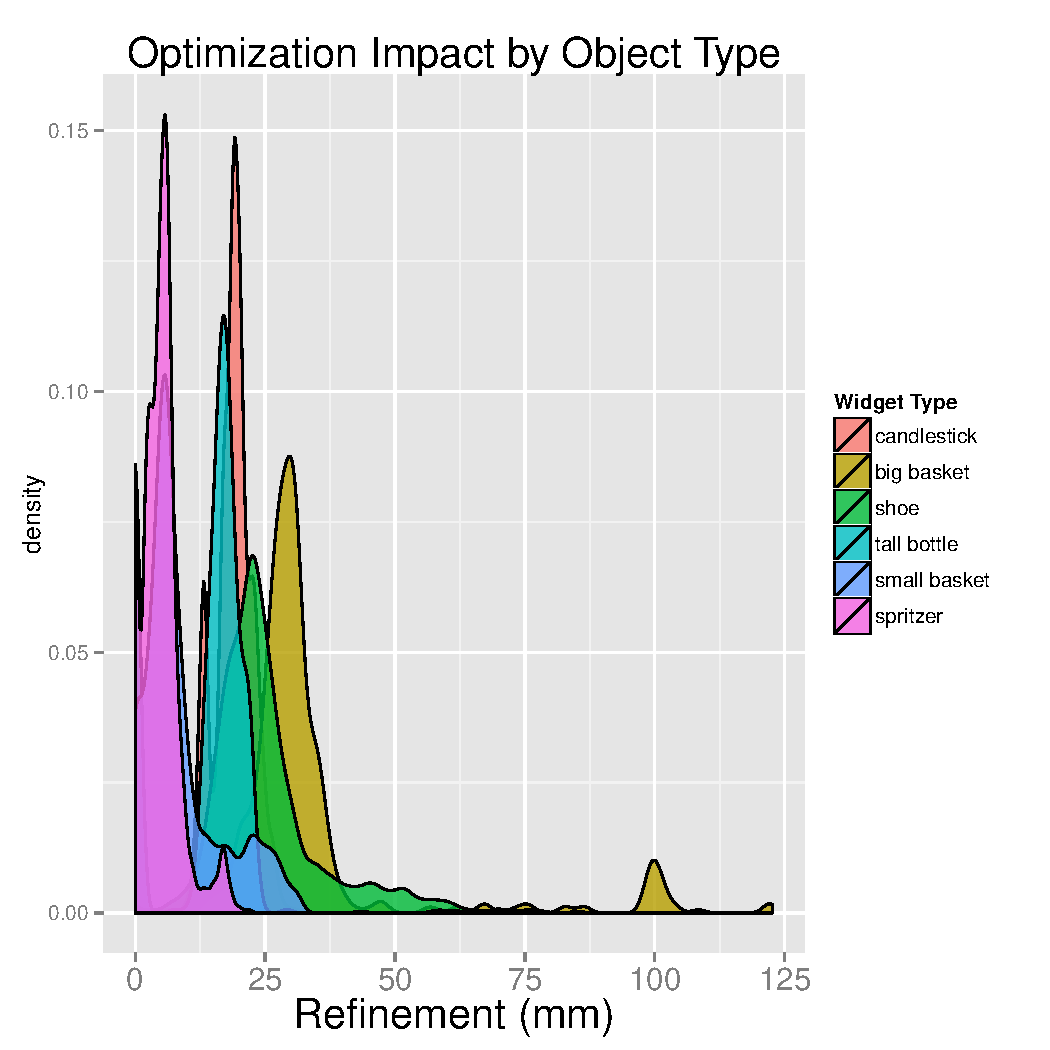
\includegraphics[width=\columnwidth]{figures/refinement.pdf}
\caption{
A nonlinear optimization that fits observed points to a per-object
cost function refines an initial localization estimate provided by
each point cluster's centroid.
}
\label{fig:refinement}
\end{figure}

The localization step begins by considering the centroid of each
cluster of points found above the table surface. This is a reasonably
good estimate of the object's position, but is biased towards the
camera due to self-occlusion of the object geometry. The goal of
navigating the PR2's finger into an opening with approximately
\unit[1]{cm} clearance on either side (e.g. underneath a spritzer
bottle's trigger) demands a level of accuracy in object pose
estimation which can be difficult to achieve when using only point
cluster centroids. However, the localization refinement step
represents a significant fraction of all the time spent in perception,
so its utility is of interest. Recovering object yaw is critical for
grasping asymmetric objects, but focusing solely on translational pose
estimation reveals further contributions made by refining initial
coarse position estimates.

Figure~\ref{fig:refinement} illustrates the translation corrections
made by the optimizer to an initial localization estimate based on
point cluster centroids with a kernel density estimate of observed
refinements. Note that in this run of experiments, there were no false
identifications and no wild misses by the robot. The two object types
needing the greatest correction from their initial centroid estimates
were the big basket and the shoe, which are the two objects with the
greatest asymmetry in the XY plane. The big basket is also a tall
object, resulting in views looking down the table that primarily see
the near side of the object. In contrast, most of the perimeter of an
item like the small basket could be seen at the available view
angle. This contrast is borne out by the effect of the optimization on
these two objects: the big basket's translational position was shifted
an average of \unit[3.4]{cm} from the point cluster centroid, while the small
basket was shifted an average of \unit[0.9]{cm}.

% \begin{table}[t]
% \centering
% \begin{tabular}{|c|c|}
% \hline
% Perception Stage & Mean Time (ms)\\ \hline \hline
% Table Extraction & 39.0 \\ \hline\hline
% Cloud Clustering & 22.2 \\ \hline
% Localization & 31.1 \\ \hline
% Total Perception & 53.2 \\ \hline
% \end{tabular}
% \caption{Perception Timing}
% \label{tab:perception-timing}
% \end{table}

\begin{figure}[t]
\centering
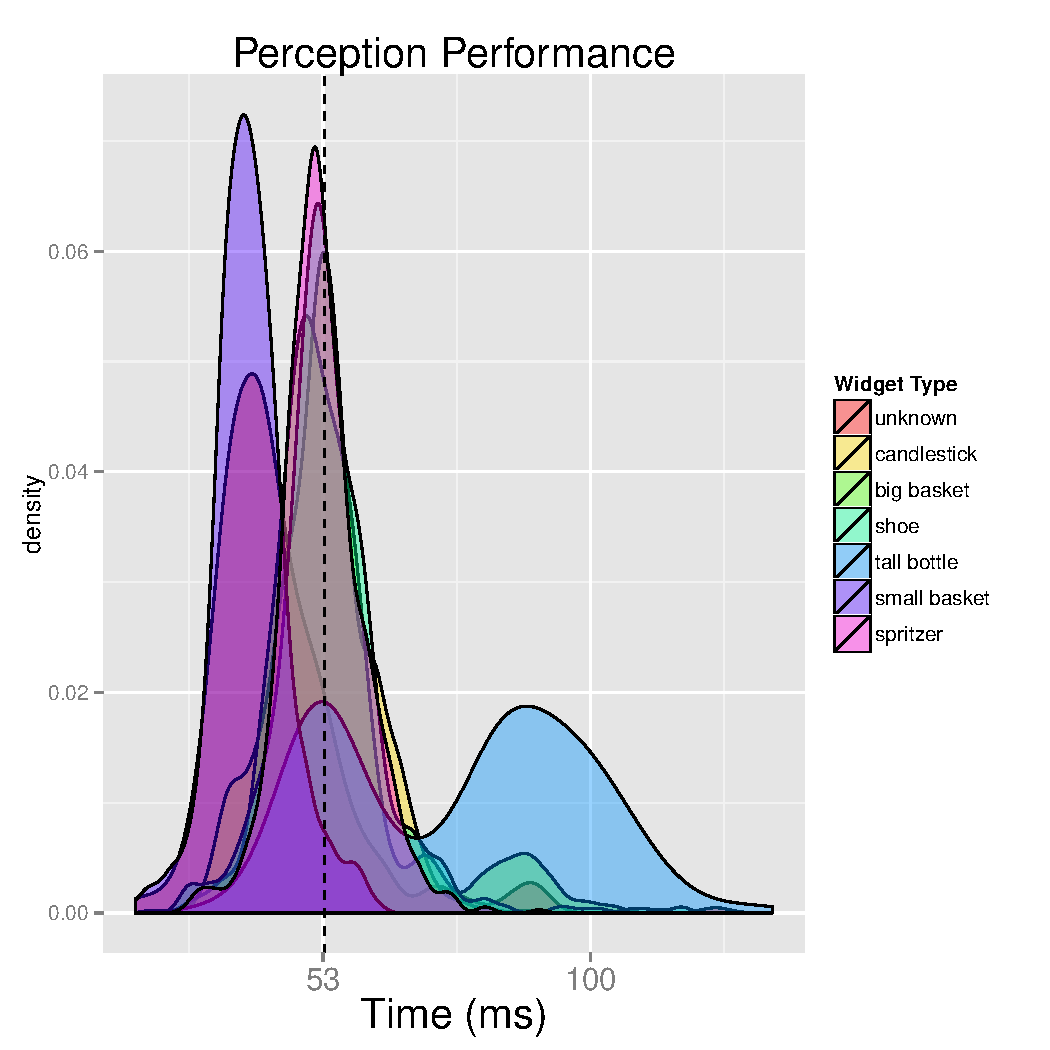
\includegraphics[width=\columnwidth]{figures/perception-density.pdf}
\caption{ Perception performance broken down by object type. The
  overall mean is \unit[53]{ms}.  }
\label{fig:perception-density}
\end{figure}

The average processing time for the perception system over the 5117
object detections during the moving object experiment was
\unit[53]{ms}, Figure~\ref{fig:perception-density}. The ``\textit{tall
  bottle}'' object was the slowest to process, at an average of
\unit[77]{ms} per update. Initial filtering, clustering, and coarse
recognition comprise the first perception phase, taking an average of
\unit[22.2]{ms}. The second phase consists of the localization
optimization procedure, taking an average of \unit[31.1]{ms}. The
final tracking phase did not take a significant amount of time.

The average processing time for the motion planner during the moving
object experiment was \unit[182]{ms}, including time spent in ROS
service calls. This gives a minimum system response time on the order
of \unit[250]{ms} if only one observation of a scene is needed. For
applications such as dynamic object manipulation, multiple
observations may be needed, which pushes the delay before action to
over \unit[400]{ms}. The performance of these experiments is thus
completely dominated by the speed at which the PR2 can move its
arms. The PR2 requires approximately \unit[4.5]{s} to perform the
motions needed for these tasks, which puts a lower limit on how
quickly the entire system can process pick-and-place tasks.

\subsection{Robustness}
Execution time -- a limiting factor in system responsiveness -- was
consistent throughout the experiments described. The longest single
perception update in the dynamic test covering 5117 updates took
\unit[132]{ms}. There are many sources of variance in these timings as
the perception system was running on the GHC Haskell runtime system
with its generational garbage collector, which itself was running in a
desktop Linux environment (Ubuntu 10.04).

Localization accuracy was measured by considering the PR2's effective
``hand-eye coordination.'' We used the PR2's proprioception to obtain
an estimate of the location of one of the robot's fingertips with its
arm extended over the work surface and angled down so that the finger
just touched the surface. The location of this tangent was marked, and
the arm was removed from the work area. A candidate object was then
placed at the marked location, and the localization returned by the
perception system was compared with the PR2's own estimate of where
its finger had been. 

These experiments yielded an average discrepancy between
proprioception and perception of \unit[5.3]{mm}. A meter stick was
then used to move the object one meter down the work surface from its
starting location. The robot's head was turned to face this new
location, and the output of perception was again recorded. This
relative motion estimate yielded an average discrepancy between the
meter stick and the perception system of \unit[6.7]{mm}.

The last metric recorded from the perception system was the speed of
the belt. This was estimated during the experiment by tracking objects
over time. The perception system estimated the belt speed at
\unitfrac[33.1]{cm\,}{\,s}, with a standard deviation of
\unitfrac[0.08]{cm\,}{\,s}. We were unable to obtain another
measurement of belt speed with less noise.

The reported timings include all segmentation, recognition, and
localization. There is additional overhead in the integrated system
due to running the perception calculations remotely from the PR2
itself. The net result was a ROS object detection publisher rate that
varied between 10 and \unit[12]{Hz}, the same rate at which raw depth
images were received at the perception computer.

\section{Conclusion}
We have demonstrated pick-and-place operations performed by a PR2 at a
rate of \unit[6.7]{s} per object at a 91\% success rate. Similar
operations on a moving work surface yield an 87\% success rate. Room
for improvement remains in the areas of system integration, and
end-effector customization. The speed at which the PR2's arms can move
proved to be a limiting factor in system performance, and the gripper
design was not particularly suited to absorbing the impact of moving
objects. Despite these mechanical limitations, the PR2 proved to be
capable of responsive, high throughput object manipulation.

\section{Acknowledgements}
This research was in part sponsored by the Army Research
Laboratory Cooperative Agreement Number W911NF-10-2-0016.


\bibliographystyle{IEEEtran}
\bibliography{refs}
\end{document}
